% Options for packages loaded elsewhere
% Options for packages loaded elsewhere
\PassOptionsToPackage{unicode}{hyperref}
\PassOptionsToPackage{hyphens}{url}
\PassOptionsToPackage{dvipsnames,svgnames,x11names}{xcolor}
%
\documentclass[
  sn-nature,
]{sn-jnl}


\usepackage{xcolor}
\usepackage{amsmath,amssymb}
\setcounter{secnumdepth}{-\maxdimen} % remove section numbering
\usepackage{iftex}
\ifPDFTeX
  \usepackage[T1]{fontenc}
  \usepackage[utf8]{inputenc}
  \usepackage{textcomp} % provide euro and other symbols
\else % if luatex or xetex
  \usepackage{unicode-math} % this also loads fontspec
  \defaultfontfeatures{Scale=MatchLowercase}
  \defaultfontfeatures[\rmfamily]{Ligatures=TeX,Scale=1}
\fi
\usepackage{lmodern}
\ifPDFTeX\else
  % xetex/luatex font selection
\fi
% Use upquote if available, for straight quotes in verbatim environments
\IfFileExists{upquote.sty}{\usepackage{upquote}}{}
\IfFileExists{microtype.sty}{% use microtype if available
  \usepackage[]{microtype}
  \UseMicrotypeSet[protrusion]{basicmath} % disable protrusion for tt fonts
}{}
\makeatletter
\@ifundefined{KOMAClassName}{% if non-KOMA class
  \IfFileExists{parskip.sty}{%
    \usepackage{parskip}
  }{% else
    \setlength{\parindent}{0pt}
    \setlength{\parskip}{6pt plus 2pt minus 1pt}}
}{% if KOMA class
  \KOMAoptions{parskip=half}}
\makeatother
% Make \paragraph and \subparagraph free-standing
\makeatletter
\ifx\paragraph\undefined\else
  \let\oldparagraph\paragraph
  \renewcommand{\paragraph}{
    \@ifstar
      \xxxParagraphStar
      \xxxParagraphNoStar
  }
  \newcommand{\xxxParagraphStar}[1]{\oldparagraph*{#1}\mbox{}}
  \newcommand{\xxxParagraphNoStar}[1]{\oldparagraph{#1}\mbox{}}
\fi
\ifx\subparagraph\undefined\else
  \let\oldsubparagraph\subparagraph
  \renewcommand{\subparagraph}{
    \@ifstar
      \xxxSubParagraphStar
      \xxxSubParagraphNoStar
  }
  \newcommand{\xxxSubParagraphStar}[1]{\oldsubparagraph*{#1}\mbox{}}
  \newcommand{\xxxSubParagraphNoStar}[1]{\oldsubparagraph{#1}\mbox{}}
\fi
\makeatother


\usepackage{longtable,booktabs,array}
\usepackage{calc} % for calculating minipage widths
% Correct order of tables after \paragraph or \subparagraph
\usepackage{etoolbox}
\makeatletter
\patchcmd\longtable{\par}{\if@noskipsec\mbox{}\fi\par}{}{}
\makeatother
% Allow footnotes in longtable head/foot
\IfFileExists{footnotehyper.sty}{\usepackage{footnotehyper}}{\usepackage{footnote}}
\makesavenoteenv{longtable}
\usepackage{graphicx}
\makeatletter
\newsavebox\pandoc@box
\newcommand*\pandocbounded[1]{% scales image to fit in text height/width
  \sbox\pandoc@box{#1}%
  \Gscale@div\@tempa{\textheight}{\dimexpr\ht\pandoc@box+\dp\pandoc@box\relax}%
  \Gscale@div\@tempb{\linewidth}{\wd\pandoc@box}%
  \ifdim\@tempb\p@<\@tempa\p@\let\@tempa\@tempb\fi% select the smaller of both
  \ifdim\@tempa\p@<\p@\scalebox{\@tempa}{\usebox\pandoc@box}%
  \else\usebox{\pandoc@box}%
  \fi%
}
% Set default figure placement to htbp
\def\fps@figure{htbp}
\makeatother





\setlength{\emergencystretch}{3em} % prevent overfull lines

\providecommand{\tightlist}{%
  \setlength{\itemsep}{0pt}\setlength{\parskip}{0pt}}





%%%% Standard Packages

\usepackage{graphicx}%
\usepackage{multirow}%
\usepackage{amsmath,amssymb,amsfonts}%
\usepackage{amsthm}%
\usepackage{mathrsfs}%
\usepackage[title]{appendix}%
\usepackage{xcolor}%
\usepackage{textcomp}%
\usepackage{manyfoot}%
\usepackage{booktabs}%
\usepackage{algorithm}%
\usepackage{algorithmicx}%
\usepackage{algpseudocode}%
\usepackage{listings}%

%%%%

\raggedbottom
\makeatletter
\@ifpackageloaded{caption}{}{\usepackage{caption}}
\AtBeginDocument{%
\ifdefined\contentsname
  \renewcommand*\contentsname{Table of contents}
\else
  \newcommand\contentsname{Table of contents}
\fi
\ifdefined\listfigurename
  \renewcommand*\listfigurename{List of Figures}
\else
  \newcommand\listfigurename{List of Figures}
\fi
\ifdefined\listtablename
  \renewcommand*\listtablename{List of Tables}
\else
  \newcommand\listtablename{List of Tables}
\fi
\ifdefined\figurename
  \renewcommand*\figurename{Figure}
\else
  \newcommand\figurename{Figure}
\fi
\ifdefined\tablename
  \renewcommand*\tablename{Table}
\else
  \newcommand\tablename{Table}
\fi
}
\@ifpackageloaded{float}{}{\usepackage{float}}
\floatstyle{ruled}
\@ifundefined{c@chapter}{\newfloat{codelisting}{h}{lop}}{\newfloat{codelisting}{h}{lop}[chapter]}
\floatname{codelisting}{Listing}
\newcommand*\listoflistings{\listof{codelisting}{List of Listings}}
\makeatother
\makeatletter
\makeatother
\makeatletter
\@ifpackageloaded{caption}{}{\usepackage{caption}}
\@ifpackageloaded{subcaption}{}{\usepackage{subcaption}}
\makeatother
\usepackage{bookmark}
\IfFileExists{xurl.sty}{\usepackage{xurl}}{} % add URL line breaks if available
\urlstyle{same}
\hypersetup{
  pdftitle={Orchestrating Microbiome Analysis with Bioconductor},
  pdfauthor={Tuomas Borman; Giulio Benedetti; Geraldson Muluh; Aura Raulo; Benjamin Valderamma; Artur Sannikov; Stefanie Peschel; Yihan Liu; Mia Contributors; Katariina Pärnänen; Christian L. Müller; Aki Havulinna; Sudarshan Shetty; Marcel Ramos; Domenick J. Braccia; Héctor Corrada Bravo; Felix M. Ernst; Levi Waldron; Thomaz Bastiaanssen; Himel Mallick; Leo Lahti},
  pdfkeywords={microbiome, Bioconductor, data science, data
integration},
  colorlinks=true,
  linkcolor={blue},
  filecolor={Maroon},
  citecolor={Blue},
  urlcolor={Blue},
  pdfcreator={LaTeX via pandoc}}


\title[Orchestrating Microbiome Analysis with
Bioconductor]{Orchestrating Microbiome Analysis with Bioconductor}

% author setup
\author*[1]{\fnm{Tuomas} \sur{Borman}}\email{tvborm@utu.fi}\author[1]{\fnm{Giulio} \sur{Benedetti}}\equalcont{These authors contributed equally to this work.}\author[1]{\fnm{Geraldson} \sur{Muluh}}\equalcont{These authors contributed equally to this work.}\author[1]{\fnm{Aura} \sur{Raulo}}\author[2]{\fnm{Benjamin} \sur{Valderamma}}\author[1]{\fnm{Artur} \sur{Sannikov}}\author[4]{\fnm{Stefanie} \sur{Peschel}}\author[5]{\fnm{Yihan} \sur{Liu}}\author[1]{\fnm{Mia} \sur{Contributors}}\author[1,6]{\fnm{Katariina} \sur{Pärnänen}}\author[1]{\fnm{Christian L.} \sur{Müller}}\author[1]{\fnm{Aki} \sur{Havulinna}}\author[]{\fnm{Sudarshan} \sur{Shetty}}\author[9]{\fnm{Marcel} \sur{Ramos}}\author[10]{\fnm{Domenick J.} \sur{Braccia}}\author[11]{\fnm{Héctor Corrada} \sur{Bravo}}\author[12]{\fnm{Felix M.} \sur{Ernst}}\author[13]{\fnm{Levi} \sur{Waldron}}\author[14]{\fnm{Thomaz} \sur{Bastiaanssen}}\equalcont{These authors contributed equally to this work.}\author[1]{\fnm{Himel} \sur{Mallick}}\equalcont{These authors contributed equally to this work.}\author*[1]{\fnm{Leo} \sur{Lahti}}\email{lemila@utu.fi}
% affil setup
\affil[1]{\orgdiv{Department of Computing}, \orgname{University of
Turku}}
\affil[1]{}
\affil[2]{\orgdiv{Department of Y}, \orgname{Organization XK}}
\affil[4]{, \orgname{Organization D}}
\affil[5]{\orgdiv{Department of
Y}, \orgname{Cornell}, \orgaddress{\street{Address}, \city{City}, \postcode{0}}}
\affil[6]{\orgdiv{Department of XYZ}, \orgname{University of Helsinki}}
\affil[9]{\orgdiv{Department of Y}, \orgname{Organization
X}, \orgaddress{\street{Address}, \city{City}, \postcode{0}}}
\affil[10]{\orgdiv{Department of Y}, \orgname{Organization
XA}, \orgaddress{\street{Address}, \city{City}, \postcode{0}}}
\affil[11]{\orgdiv{Department of YS}, \orgname{Organization
XP}, \orgaddress{\street{Address}, \city{City}, \postcode{0}}}
\affil[12]{\orgdiv{Department of Y}, \orgname{Organization
XB}, \orgaddress{\street{Address}, \city{City}, \postcode{0}}}
\affil[13]{\orgdiv{Department of Y}, \orgname{Organization
N}, \orgaddress{\street{Address}, \city{City}, \postcode{0}}}
\affil[14]{\orgdiv{Department of Y}, \orgname{Organization XX}}

% abstract 

\abstract{The expansion of microbiome research has led to the
accumulation of interlinked datasets encompassing versatile taxonomic
and functional assays. While critical to advance the field, the analysis
of increasingly large and heterogeneous multi-modal microbiome data
would benefit from unified approaches supporting interoperability
between methods and the design of modular data science workflows. The
Bioconductor project has recently developed an optimized statistical
programming framework for multi-assay data integration in computational
life sciences. Building on this foundation, we introduce a
community-developed open-source ecosystem for microbiome data science,
dedicated to supporting joint analysis of hierarchical, interlinked, and
heterogeneous datasets that are increasingly common in modern microbiome
research. This interoperable infrastructure comprises of open-source
datasets, methods, tutorials and an active online community. Its
functionality and usage are detailed in the OMA book
(https://microbiome.github.io/OMA/docs/devel), which offers guidance for
prospective users and contributors.}

% keywords
\keywords{microbiome,  Bioconductor,  data science,  data integration}

\begin{document}
\maketitle


\section{Introduction}\label{sec-intro}

Modern data science applications critically rely on open-source methods
created by the research community \citep{Barker2022, Pearson2025} and
open software ecosystems have become central innovation hubs, driving
technological and cultural transformation \citep{Hocquet2024}. The
Bioconductor project has been established as a major distribution
channel for open data science methods in the life sciences. Nowadays,
its vast developer community maintains over 2,300 quality-controlled R
packages for various fields of life science informatics
\citep{gentleman2004}. Additionally, Bioconductor has evolved into a
global community that supports data science collaboration and training
\citep{drnevich2025} in general, and now the international calls for
enhancing microbiology education in particular \citep{Timmis2024}.

Microbiome research focuses on the study of microbial communities and
their diversity, function, and interactions with the host and
environment \citep{moreno-indias2021}. The technologies used in this
field generate vast amounts of high-dimensional, hierarchically
structured data. The expansion of microbiome research has led to the
accumulation of interlinked, multi-modal datasets encompassing versatile
taxonomic and functional assays. Microbiome data scientists are thus
increasingly facing the need to integrate heterogeneous data across
multiple modalities while implementing reproducible workflows, which
presents many practical challenges. First, the unique statistical
properties and complexity of microbiome data necessitate specialized
approaches \citep{moreno-indias2021, Jeganathan2021, Willis2019}.
Secondly, the diversity of proposed solutions can make it difficult to
identify the optimal methods and build interoperable workflows
\citep{Wen2023, Shetty2019}. Thus, the need for standardized microbiome
data science infrastructures has been widely recognized
\citep{moreno-indias2021} and a variety of open microbiome data science
frameworks have been developed, including Anvi'o \citep{Eren2021},
Mothur \citep{schloss2009}, QIIME2 \citep{bolyen2019}, and phyloseq
\citep{mcmurdie2012}. However, platforms that exclusively focus on
microbiome data science may not be able to optimally address the need to
link data across different multiple modalities originating from
different research domains.

The Bioconductor project embeds the methods of microbiome data science
into a wider statistical programming framework alongside with the
concurrent development of interoperable methods and workflows for
transcriptomics \citep{righelli2022}, single-cell \citep{amezquita2020},
metabolomics \citep{gatto2025}, proteomics \citep{gatto2025, Anwar2025},
and other fields. Here, we introduce a community-developed open-source
framework, supporting multi-modal data integration in microbiome
research. We have extensively tested and documented the framework to
facilitate the dissemination of evidence-based best practices in
microbiome data science.

\section{Data infrastructure}\label{sec-infra}

Data scientists routinely deal with interlinked assays, side
information, and hierarchical data such as ontologies, trees, or
networks. The ability to integrate heterogeneous data elements is
essential in biological research, where the individual components of a
system can be seldom studied in isolation. The challenge for a data
scientist is that different methods often require variable and
inconsistent input data formats, leading to technical complications and
time lost on repeated data wrangling during routine analyses.
Bioconductor is renowned for its ecosystem of interoperable statistical
methods for life sciences. A key to its broad adoption has been its
ability to mitigate those issues by providing standardized data
structures supported by an ecosystem of interoperable methods. This
helps to avoid wrangling data and aligning methods and leaves more time
to be invested in the core analytical tasks.

Bioconductor data structures support statistical analysis of complex
data combinations \citep{huber2015} and are widely adopted by various
user communities. They have been implemented through specialized
object-oriented classes that integrate multiple data elements into a
single structure known as \emph{data container} \citep{chambers2014}.
The SummarizedExperiment (SE) class represents the primary data
container underlying the Bioconductor ecosystem
\citep{huber2015, morgan2025}. Its position among the top-1\% most
downloaded packages in Bioconductor reflects its widespread recognition
and increasing adoption among developers
(Figure~\ref{fig-bioc_packages}). SE provides a standardized solution to
store tabular data by linking numeric abundance matrices with side
information on features (rows) and samples (columns). Side information
can include secondary details on the experiment, such as sample origin,
collection time, or health status.

The interoperability of SE with other Bioconductor data structures
facilitates the transfer of methods across different fields of omics
research. This represents a major strength, which has facilitated the
development of modular and scalable data science methods
\citep{drnevich2025}. The shared data structures support the transfer of
methods between omics fields, yielding improved overall quality control
and user support. Consequently, the SE-based framework has been extended
to similar data integration tasks in fields, such as single-cell and
spatial omics through the SingleCellExperiment (SCE)
\citep{amezquita2020} and SpatialExperiment \citep{righelli2022}
classes, respectively.

\begin{figure}

\centering{

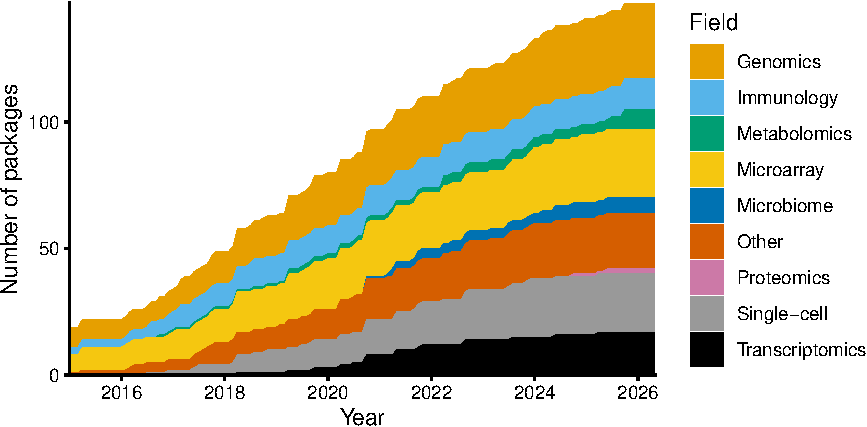
\includegraphics[width=0.7\linewidth,height=\textheight,keepaspectratio]{manuscript_files/figure-pdf/fig-bioc_packages-1.pdf}

}

\caption{\label{fig-bioc_packages}\textbf{Adoption of the
SummarizedExperiment (SE) data container among Bioconductor developers.}
The growth in the number of Bioconductor packages supporting SE over
time is shown, categorized by their respective fields. For some of the
packages SE support has been added after their original release.}

\end{figure}%

\textbf{Hierarchical data structures.} Microbiome data scientists
frequently need to\\
integrate information on feature phylogenies and sample hierarchies in
order to accurately reflect fine-scale variability in microbiome data.
While maintaining interoperability with the broader Bioconductor
ecosystem, the TreeSummarizedExperiment (TreeSE) class \citep{huang2021}
extends the SE and SCE data structures to hierarchical datasets by
incorporating feature and sample organisations as tree structures
(Figure~\ref{fig-datacontainers}). Moreover, TreeSE supports the storage
of other common aspects of microbiome data, such as reference sequences,
and incorporates results from common analytical procedures such as
dimensionality reduction, statistical transformations, and agglomeration
by taxonomic, functional or other information. The interoperability with
other Bioconductor classes facilitates scalable analysis and the design
of modular yet flexible workflows. The direct interoperability with the
widely adopted SE data science ecosystem distinguishes our TreeSE-based
approach from phyloseq, which is another popular Bioconductor data
container originally developed with a focus on 16S amplicon data
analysis \citep{mcmurdie2012}. TreeSE is a superset that can accommodate
all elements of a phyloseq object, while also offering improved support
for multi-modal data and often substantial gains in memory efficiency
and computing speed (Figure~\ref{fig-benchmarking}). Overall, the TreeSE
approach outperforms phyloseq in these benchmarks. While speedyseq is
faster in certain operations, TreeSE scales more efficiently in both
execution time (t) and allocated memory (m) as sample size (n)
increases. Conversion functions and detailed cheat sheets between the
two formats are available to bridge the gap between the respective user
communities.

\begin{figure}

\begin{minipage}{0.50\linewidth}

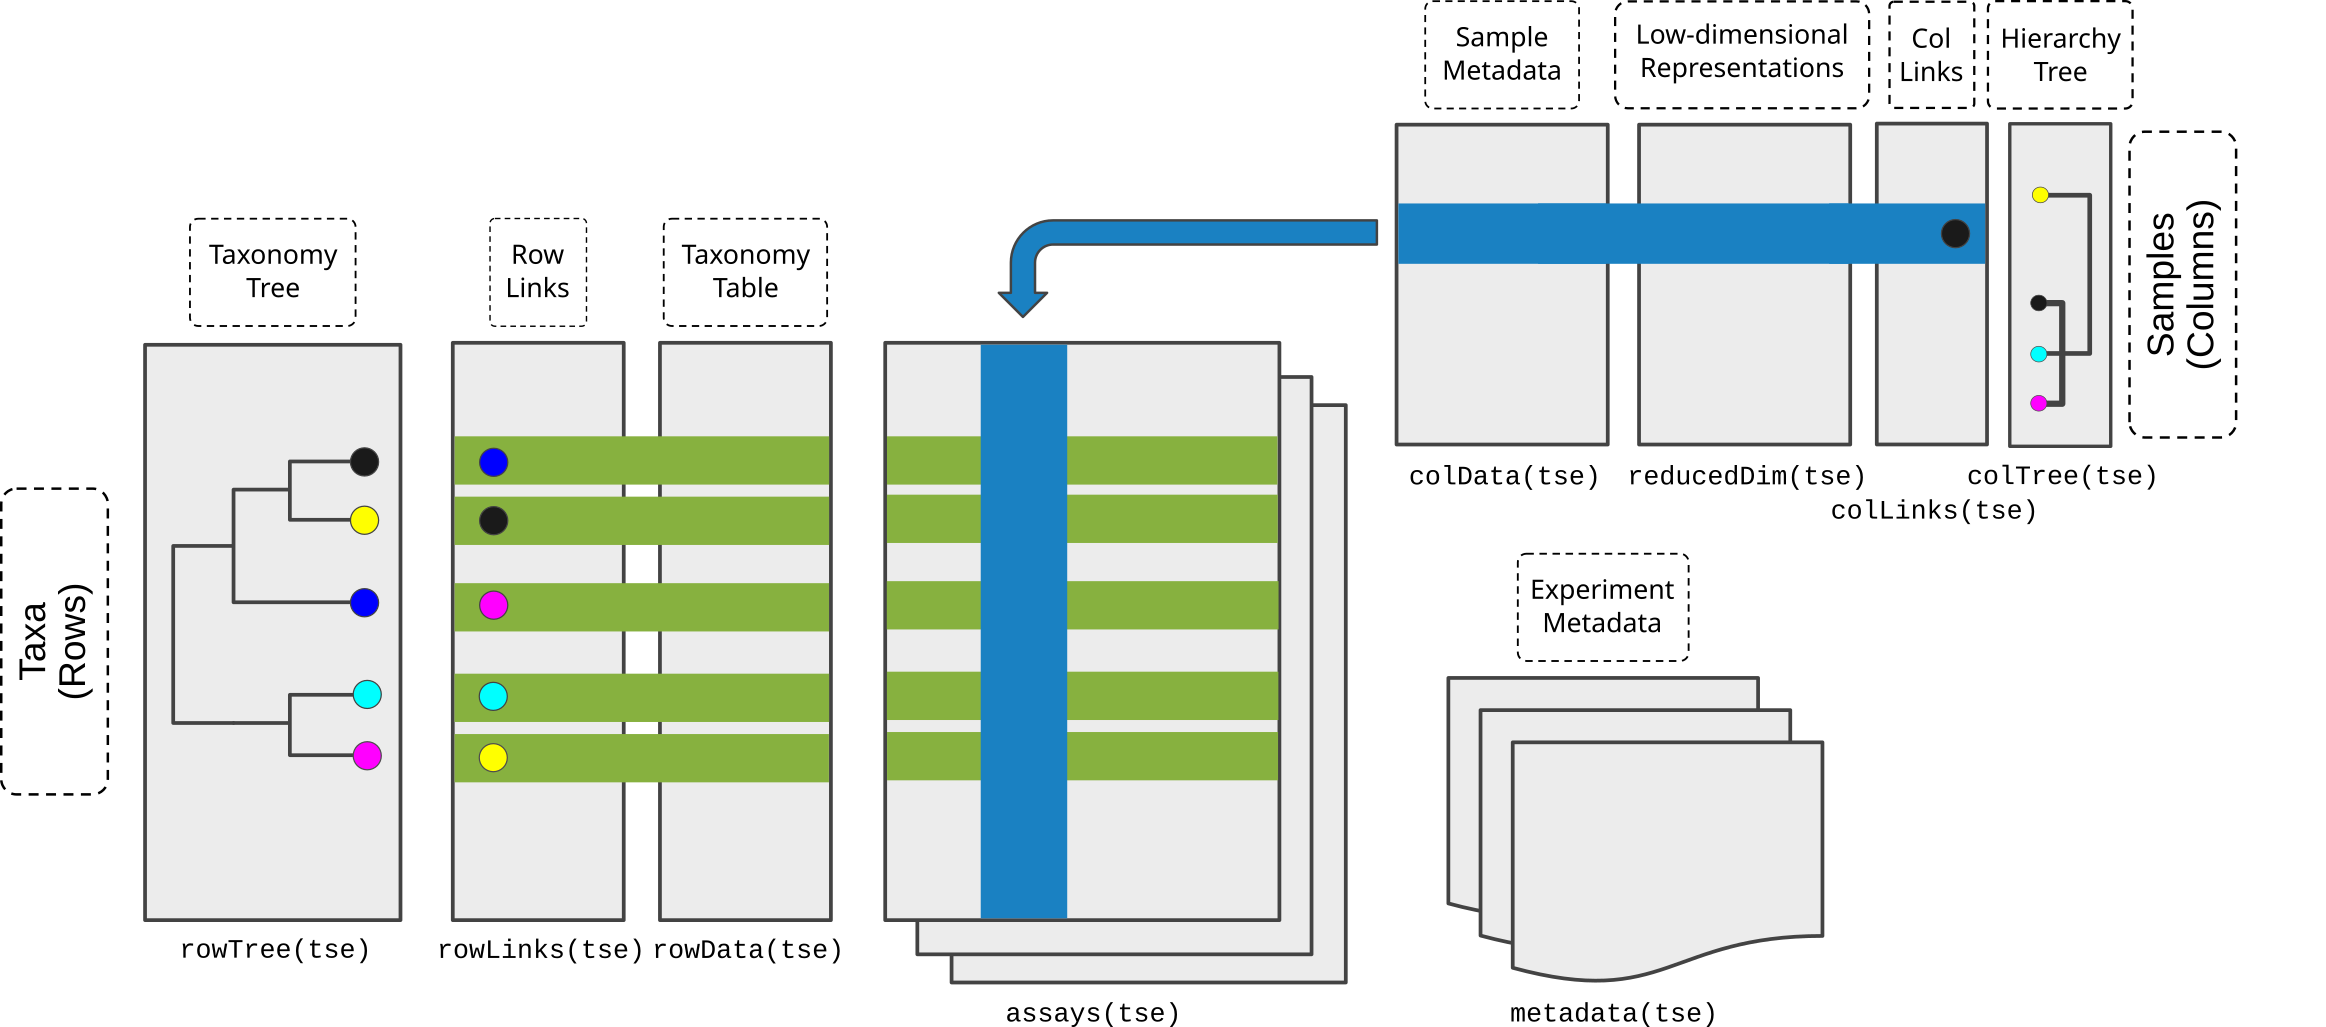
\includegraphics[width=1\linewidth,height=\textheight,keepaspectratio]{figures/TreeSE.png}

\subcaption{\label{}TreeSummarizedExperiment}
\end{minipage}%
%
\begin{minipage}{0.50\linewidth}

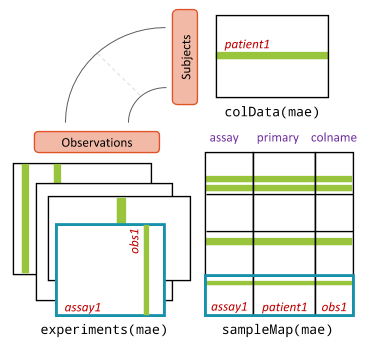
\includegraphics[width=0.6\linewidth,height=\textheight,keepaspectratio]{figures/mae.png}

\subcaption{\label{}MultiAssayExperiment}
\end{minipage}%

\caption{\label{fig-datacontainers}\textbf{\emph{Bioconductor data
containers for microbiome data.}} \textbf{(a) TreeSummarizedExperiment
(TreeSE).} TreeSE supports hierarchical and multi-table analysis in
microbiome data science \citep{huang2021}. It links the numeric
abundance matrix and potential alternative versions (statistical
transformations, different taxonomic levels, dimensionality reduction)
with tabular and hierarchical side information on the features (rows)
and samples (columns). Additional slots for reference sequences and
experiment metadata are available. \textbf{(b) MultiAssayExperiment
(MAE).} MAE facilitates integration of data from multiple experiments
\citep{ramos2017}.}

\end{figure}%

\begin{figure}

\centering{

\pandocbounded{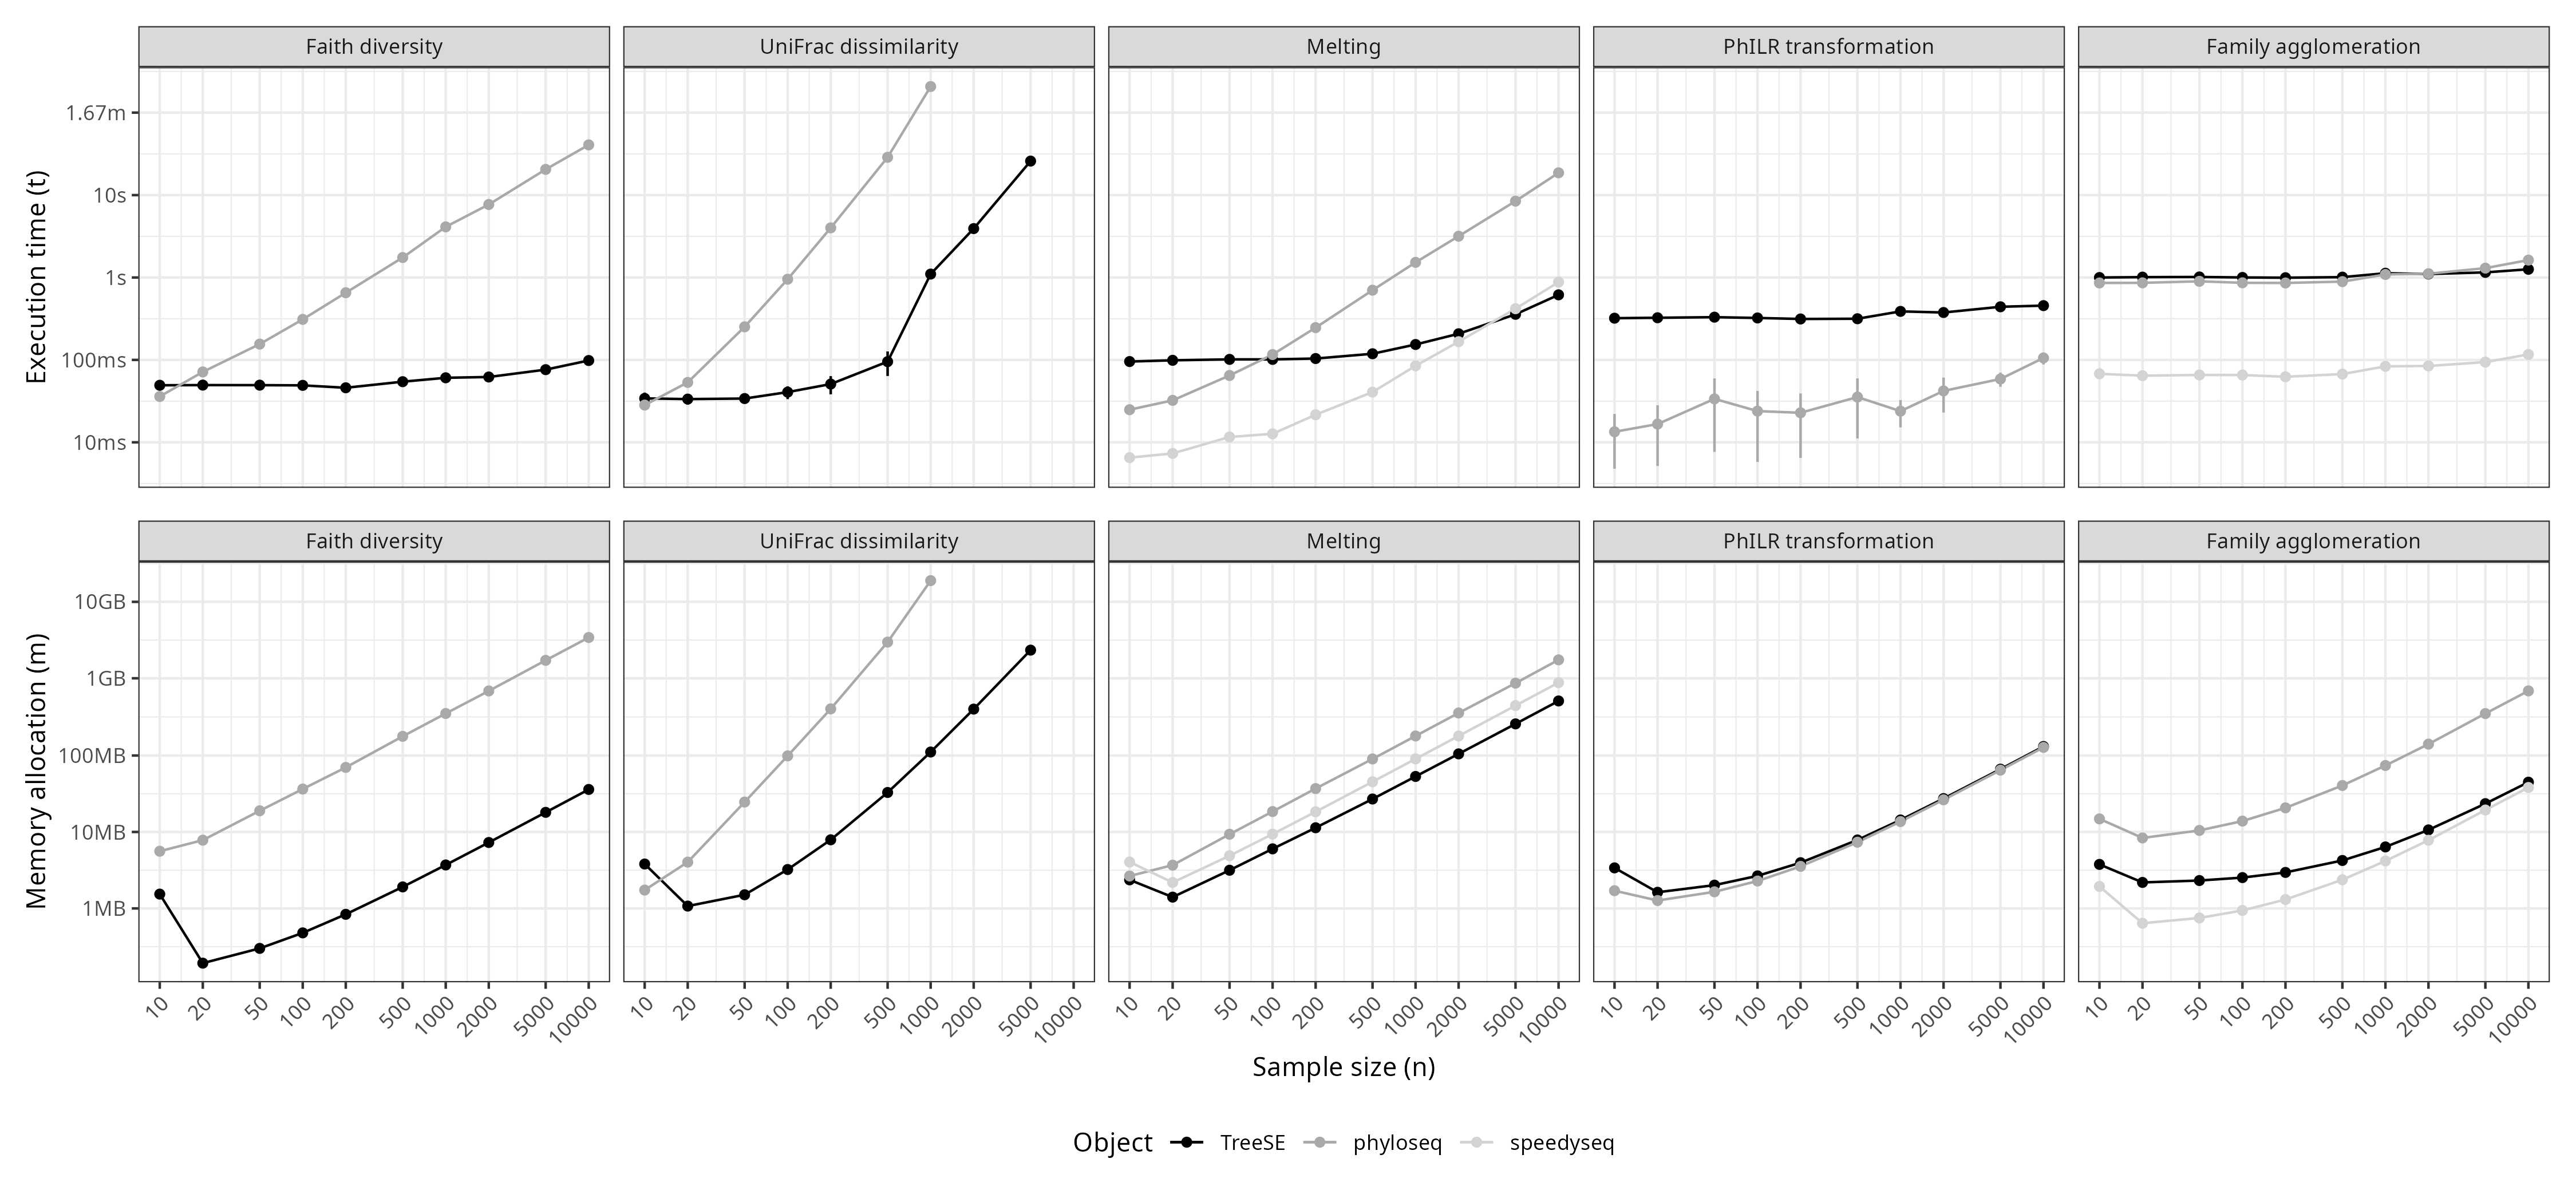
\includegraphics[keepaspectratio]{figures/benchmarking.png}}

}

\caption{\label{fig-benchmarking}\textbf{Comparison of execution time
and memory consumption between alternative methods in Bioconductor}
TreeSE, phyloseq and speedyseq were benchmarked for five common
analytical operations applied to random subsets of samples from a large
study on wild baboons \citep{Grieneisen2021} (accessible through the
microbiomeDataSets Bioconductor package). The source code for the
benchmarking experiments can be accessed through the OMA online book.}

\end{figure}%

\textbf{Multi-assay data structures.} When integrating data across
multiple modalities, such as taxonomy, metabolomics, or host genomics,
more flexible sample mapping may become necessary. Multi-omics data is
often sparse, and samples can be only partially matched between
experiments. In other cases, a single sample in one modality can be
matched by two or more samples in another modality \citep[see
e.g.][]{Husso2023}. The MultiAssayExperiment (MAE) data container
\citep{ramos2017} facilitates the integration of multiple data objects
representing different omics modalities (see
Figure~\ref{fig-datacontainers}). Whereas TreeSE is restricted to a
one-to-one sample mapping between different data tables, MAE supports
flexible mappings between multiple experiments from the same study.
Integration of multi-table data without such structured framework often
leads to ambiguous mappings and inconsistent results. For instance,
diagonal integration methods \citep{xu2022, argelaguet2021computational}
-- where shared features across data types may not be explicitly defined
-- can benefit substantially from such systematic framework that enforce
anchor alignment. This mirrors lessons from single-cell data
integration, where shared anchors and hierarchical mapping have proven
essential for interpretability. Flexible linking of samples across
several data objects supports efficient data integration, methods
sharing, and overall interoperability.

Table~\ref{tbl-containers} summarizes the microbiome-related data
containers, while Table~\ref{tbl-elements} introduces the available data
elements in each container.

\begin{longtable}[]{@{}
  >{\raggedright\arraybackslash}p{(\linewidth - 2\tabcolsep) * \real{0.5000}}
  >{\raggedright\arraybackslash}p{(\linewidth - 2\tabcolsep) * \real{0.5000}}@{}}
\caption{Recommended data containers for microbiome
analysis.}\label{tbl-containers}\tabularnewline
\toprule\noalign{}
\begin{minipage}[b]{\linewidth}\raggedright
Data container
\end{minipage} & \begin{minipage}[b]{\linewidth}\raggedright
Target use
\end{minipage} \\
\midrule\noalign{}
\endfirsthead
\toprule\noalign{}
\begin{minipage}[b]{\linewidth}\raggedright
Data container
\end{minipage} & \begin{minipage}[b]{\linewidth}\raggedright
Target use
\end{minipage} \\
\midrule\noalign{}
\endhead
\bottomrule\noalign{}
\endlastfoot
SummarizedExperiment (SE)\citep{huber2015} & generic data container for
experiments with multiple assays \\
TreeSummarizedExperiment (TreeSE)\citep{huang2021} & tailored data
container for hierarchically organized experiments \\
MultiAssayExperiment (MAE)\citep{ramos2017} & tailored data container
for sets of multi-omic experiments \\
\end{longtable}

\begin{longtable}[]{@{}
  >{\raggedright\arraybackslash}p{(\linewidth - 8\tabcolsep) * \real{0.1700}}
  >{\raggedright\arraybackslash}p{(\linewidth - 8\tabcolsep) * \real{0.6300}}
  >{\centering\arraybackslash}p{(\linewidth - 8\tabcolsep) * \real{0.0300}}
  >{\centering\arraybackslash}p{(\linewidth - 8\tabcolsep) * \real{0.0900}}
  >{\centering\arraybackslash}p{(\linewidth - 8\tabcolsep) * \real{0.0800}}@{}}
\caption{Key data elements in the employed data
containers.}\label{tbl-elements}\tabularnewline
\toprule\noalign{}
\begin{minipage}[b]{\linewidth}\raggedright
Slot
\end{minipage} & \begin{minipage}[b]{\linewidth}\raggedright
Content
\end{minipage} & \begin{minipage}[b]{\linewidth}\centering
SE
\end{minipage} & \begin{minipage}[b]{\linewidth}\centering
TreeSE
\end{minipage} & \begin{minipage}[b]{\linewidth}\centering
MAE\(^a\)
\end{minipage} \\
\midrule\noalign{}
\endfirsthead
\toprule\noalign{}
\begin{minipage}[b]{\linewidth}\raggedright
Slot
\end{minipage} & \begin{minipage}[b]{\linewidth}\raggedright
Content
\end{minipage} & \begin{minipage}[b]{\linewidth}\centering
SE
\end{minipage} & \begin{minipage}[b]{\linewidth}\centering
TreeSE
\end{minipage} & \begin{minipage}[b]{\linewidth}\centering
MAE\(^a\)
\end{minipage} \\
\midrule\noalign{}
\endhead
\bottomrule\noalign{}
\endlastfoot
\textbf{Tables} & & & & \\
assays & tables of features (rows) and samples (cols) & X & X & X \\
altExps\(^b\) & experiments with variable number of features & & X &
X \\
reducedDims & results of dimensionality reduction & & X & X \\
\textbf{Rows} & & & & \\
rowData & side information on features & X & X & X \\
rowPairs & linkage between pairs of associated features & & X & X \\
rowTrees & hierarchical organization of features & & X & X \\
referenceSeq & reference sequences of features & & X & X \\
\textbf{Columns} & & & & \\
colData & side information on samples & X & X & X \\
colTrees & hierarchical organization of samples & & X & X \\
sampleMap\(^c\) & flexible sample mapping across experiments & & & X \\
\textbf{Other} & & & & \\
metadata & additional information on the experiment & X & X & X \\
\end{longtable}

\(^a\) While MAE does not contain conventional slots (with the exception
of colData), its experiments can include any number of data containers
that provide those slots. \(^b\) altExp samples must match assay samples
in a 1-to-1 mapping. \(^c\) sampleMap supports diverse mappings between
samples from different experiments (1-to-1, 1-to-many, many-to-1 and
many-to-many).

\textbf{Data resources.} Several open data resources support this
framework for microbiome analysis and direct data import in the
aforementioned data containers for further downstream analysis in
Bioconductor. Examples of the available data resources include
curatedMetagenomicData \citep{pasolli2017}, HoloFood \citep{rogers2024},
microbiomeDataSets \citep{microbiomedatasets}, and the EBI/MGnify
database \citep{gurbich2023}. In addition, Bioconductor packages often
include built-in demonstration datasets. Collectively, these resources
encompass taxonomic and functional profiles from thousands of published
microbiome studies and tens of thousands samples that can be accessed
with the available tools for research and educational purposes (see
Table~\ref{tbl-dataresources}).

\begin{longtable}[]{@{}
  >{\raggedright\arraybackslash}p{(\linewidth - 6\tabcolsep) * \real{0.3000}}
  >{\raggedright\arraybackslash}p{(\linewidth - 6\tabcolsep) * \real{0.4000}}
  >{\raggedright\arraybackslash}p{(\linewidth - 6\tabcolsep) * \real{0.1500}}
  >{\raggedright\arraybackslash}p{(\linewidth - 6\tabcolsep) * \real{0.1500}}@{}}
\caption{Open microbiome data resources supporting the
framework.}\label{tbl-dataresources}\tabularnewline
\toprule\noalign{}
\begin{minipage}[b]{\linewidth}\raggedright
Data resource
\end{minipage} & \begin{minipage}[b]{\linewidth}\raggedright
Package
\end{minipage} & \begin{minipage}[b]{\linewidth}\raggedright
\# studies or datasets
\end{minipage} & \begin{minipage}[b]{\linewidth}\raggedright
\# samples
\end{minipage} \\
\midrule\noalign{}
\endfirsthead
\toprule\noalign{}
\begin{minipage}[b]{\linewidth}\raggedright
Data resource
\end{minipage} & \begin{minipage}[b]{\linewidth}\raggedright
Package
\end{minipage} & \begin{minipage}[b]{\linewidth}\raggedright
\# studies or datasets
\end{minipage} & \begin{minipage}[b]{\linewidth}\raggedright
\# samples
\end{minipage} \\
\midrule\noalign{}
\endhead
\bottomrule\noalign{}
\endlastfoot
Curated metagenomic data \citep{pasolli2017} & curatedMetagenomicData
\citep{pasolli2017} & 93 & 22,588 \\
HoloFood \citep{rogers2024} & HoloFoodR \citep{holofoodr} & - & 9,990 \\
MGnify \citep{gurbich2023} & MGnifyR \citep{mgnifyr} & 5129 & 616,138 \\
microbiomeDataSets \citep{microbiomedatasets} & microbiomeDataSets
\citep{microbiomedatasets} & 6 & 19,100 \\
\end{longtable}

\section{Data preparation}\label{sec-process}

While microbiome data scientists continue to develop specialized
solutions \citep{Jeganathan2021, Willis2019, MarcosZambrano2023}, the
implementations typically differ in their expected input and output
formats. Common data standards support modular data science workflows,
speeding up methods development, benchmarking, and replication. Here, we
describe an ecosystem of software packages that has recently emerged to
support microbiome data integration and analysis based on the data
containers, (Tree)SE and MAE (see Figure~\ref{fig-workflow}).

The framework focuses primarily on the downstream analysis of
high-throughput sequencing data from microbiome experiments after the
original measurements have already been summarized into abundance tables
representing e.g.~taxonomic or functional profiles. Taxonomic abundance
tables are one of the most commonly encountered data types. Common
measurement platforms include amplicon-based marker gene studies
(e.g.~16S rRNA) and metagenomic sequencing, but alternative profiling
techniques are available including phylogenetic microarrays
\citep{RajilicStojanovic2009} and high-density optical mapping
\citep{Abakumov2024}. Microbiome analyses can also yield variable
metagenomic, and functional features. The interoperability of the data
formats supports modular workflow design for integrating different omics
through the Bioconductor ecosystem. This decisively mitigates
reproducibility challenges posed by rapidly evolving reference databases
and profiling tools (e.g., MetaPhlAn2 vs.~MetaPhlAn4) by enabling
structured coexistence and direct comparison within a unified,
version-resilient framework \citep{blanco2023, truong2015}.

\textbf{Data import.} Most users will need to import data for their own
analyses. The TreeSE data container can be populated with microbiome
data from common tabular data types but non-standard file formats may
require additional, custom data wrangling as usual. To streamline data
import, we provide importers for a variety of standard microbiome file
formats including BIOM \citep{mcdonald2012}, MetaPhlAn/HUMAnN (MetaPhlAn
v. 2-4, HUMAnN v. 3) \citep{mciver2017}, Mothur \citep{schloss2009},
QIIME2 \citep{bolyen2019} and the TAXonomic Profile Aggregation and
STAndardisation format (taxpasta) \citep{beber2023}. These importers can
automatically load the data into the appropriate data containers, thus
forming a bridge between low-level sequence processing methods and the
high-level statistical programming framework in R. Moreover, converters
between alternative data structures in R are available supporting
seamless conversions between TreeSE and BIOM, DADA2 \citep{callahan2016}
and phyloseq (the mia::convert* functions), and TreeSE-based microbiome
data objects can be exported into external services such as MicrobiomeDB
\citep{Oliveira2018} and in other languages (e.g.~Julia). These bridges
facilitate the broadest possible access to microbiome analysis methods.

\textbf{Quality control and exploration.} After importing the data in R,
the recommended first step involves basic data exploration and quality
control \citep{zuur2010}. In addition to methods for identifying
contaminant sequences and calculating summary statistics, the framework
includes a versatile set of custom visualization methods to assess data
variability, outliers, homogeneity of variance and other aspects that
may need to be considered in downstream data analysis. The mia and
miaViz packages, for instance, provide convenient access to many
operations for common exploratory tasks in microbiome analysis and
visualization for TreeSE objects (Figure~\ref{fig-downstream_analyses}).

\textbf{Filtering and agglomeration.} Microbiome datasets may contain
tens of thousands of unique features depending on the sequencing
resolution, databases, and the scope of analysis. Often -- to summarize
data into biologically meaningful groups or to reduce multiple
comparisons -- the data is subsetted, filtered or agglomerated to
higher-level taxonomic or functional categories or stratified by sample
groups. The package ecosystem and the mia package feature various tools
for such tasks. For instance, the prevalence methods can be useful to
remove very rare features that might be sequencing artifacts or present
otherwise limited value for the analysis. The mechanism of alternative
experiments (altExp) supports data agglomeration by taxonomic levels and
by other features such as pathogeneicity or functional potential
(e.g.~butyrate production \citep{Kullberg2024}, gut-brain modules
\citep{VallesColomer2019}, and other host-associated signatures
\citep{geistlinger2024}). The supporting methods incorporate the
agglomerated levels within the same data object for parallel operations,
and typically also take care of agglomerating the associated tree
information and the alternative assays. The filtering, subsetting, and
agglomeration operations are thus supported in both feature as well as
sample spaces, and simultaneously propagate to cover the relevant
alternative assays, alternative experiments, ordinations, and side
information. This supports the efficient management of interlinked
assays and saves time for dedicated expert tasks.

\textbf{Transformation.} Data transformations are frequently encountered
in statistical analysis. Common transformations in microbiome research
include the relative abundance \citep{gloor2017}, centered log-ratio
(CLR) and its robust version (rCLR), which are used to mitigate
compositionality bias \citep{Martino2019}, and the tree-aware
phylogenetic ILR (phILR) transformation \citep{silverman2017}. Data
rarification is a related concept that has been suggested to control for
uneven sequencing depths and it remains widely debated in microbial
ecology \citep{mcmurdie2014, schloss2024}. Our framework supports these
and a variety of other transformations commonly applied to microbiome
data.

\textbf{Data enrichment.} Finally, incorporating additional data is a
frequent operation in applied data analysis, and it often takes place in
an iterative fashion. The data containers support gradual and organized
accumulation of interlinked data elements including transformations,
aggregated data, dimension reduction, and derived data on samples and
features. We generally recommend that the data objects are initialized
at the beginning of the workflow, where they can then be gradually
enriched as the project advances. By systematically extending the
upstream data preparation step -- instead of ad-hoc calculations
scattered along the workflow -- the data scientist can achieve
well-organized and transparent provenance of the data elements. Data can
be enriched by importing new external information as well as by deriving
new information from the data itself into the same data container as
described in the next section.

\begin{figure}

\centering{

\pandocbounded{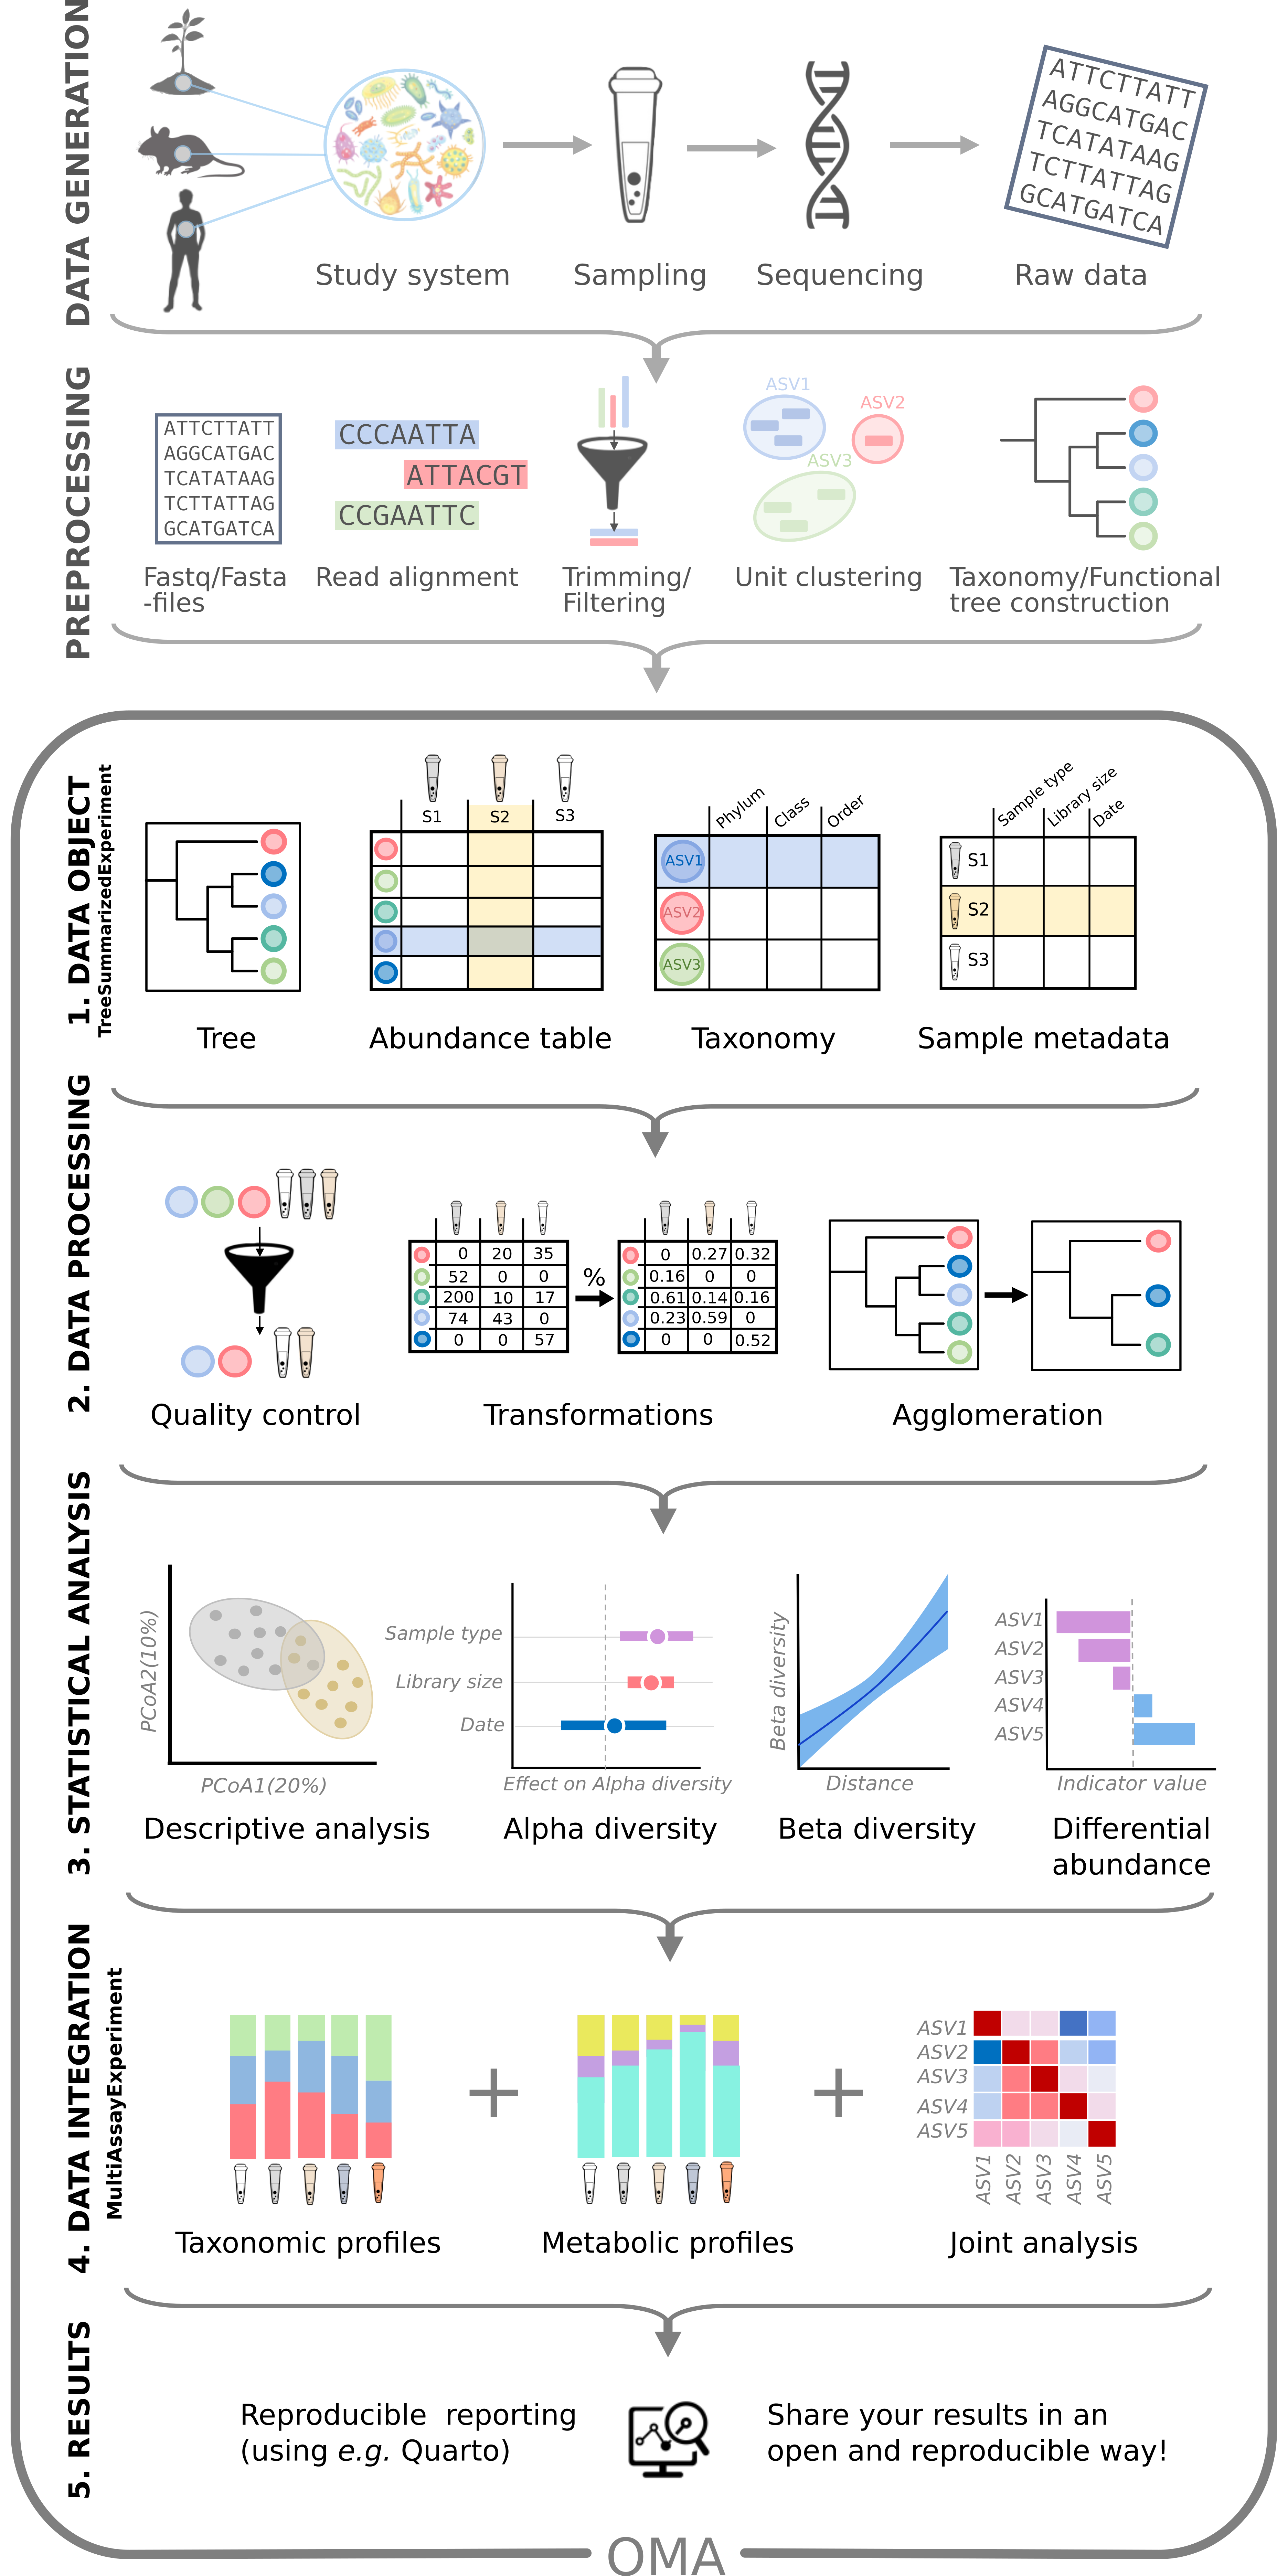
\includegraphics[keepaspectratio]{figures/workflow.png}}

}

\caption{\label{fig-workflow}\textbf{Examples of Bioconductor tools
along the microbiome data science workflow.} A typical microbiome
workflow starts with taxonomic and functional annotation. The processed
microbiome data can then be imported to Bioconductor data container
(TreeSE), or integrated with other omics using the MAE container for
downstream statistical analysis. (Figure adapted from
\citep{amezquita2020})}

\end{figure}%

\section{Downstream data analysis}\label{sec-analysis}

The new analysis framework improves the management of analysis workflows
by systematically linking the different data elements and analysis
outcomes. The framework is thus shifting the focus towards multi-modal
analyses and methods development while at the same time supporting the
essential standard techniques in microbiome research, such as community
diversity and composition. Microbiome data analysis often relies on
specialized statistical approaches as data sparsity, zero-inflation,
compositionality, and heteroschedasticity pose challenges for standard
data analytical methods \citep{gloor2017, Jeganathan2021}. Moreover,
microbiome data is hierarchically structured across taxonomic,
ecological, and spatial levels \citep{moreno-indias2021, Ruuskanen2021}.
Alternative processing pipelines pose different biases and generate
varying data formats \citep{quince2017}. These and other unique
characteristics have wide-reaching implications for downstream analysis,
necessating dedicated processing and analysis methods in microbiome
research \citep{moreno-indias2021}. Our statistical programming
framework supports the community-driven development and benchmarking of
these solutions. The following sections provide an overview of the
available tools for microbiome data science.

\textbf{Community indicators.} Various global indicators are available
to quantify the microbial community state or other sample properties.
Community diversity represents a common measure in microbial ecology
\citep{bastiaanssen_bugs1_2023} (Figure~\ref{fig-downstream_analyses}).
Alpha diversity metrics generally quantify the observed or estimated
number of distinct species (``richness'') and their distribution
(``evenness''). Many diversity indices, such as the Shannon index,
combine these two aspects. Phylogenetic diversity measures additionally
consider the phylogenetic relatedness of community members
\citep{faith1992}; the new implementation of the Stacked Faith's
Phylogenetic Diversity can accelerate the performance 1-2 orders of
magnitude \citep{Armstrong2021}. Enhanced analyses with repeated
rarefaction are supported \citep{Schloss2024b} albeit the use of
rarefaction remains controversial \citep{schloss2024, Willis2019b}.
Other global indices of community state include measures of dominance,
rarity, skewness, kurtosis, modality, library size (number of reads), or
absolute abundance quantification. Sample information in the TreeSE
object (colData) can be enriched with these derived quantities. By
default, the mia::addAlpha method returns a set of complementary alpha
diversity measures \citep{Cassol2025}.

\textbf{Community similarity} is commonly evaluated with beta diversity
measures, which quantify multivariate dissimilarity and can be used to
quantitatively comparecommunity composition. The framework supports
common indices in microbial ecology including Bray-Curtis, Jaccard, and
Aitchison \citep{bastiaanssen_bugs1_2023, Martino2019}, and the
phylogeny-aware UniFrac \citep{lozupone2005}. The community
(dis)similarities are commonly visualized with unsupervised ordination
methods that project the data on a lower-dimensional display
\citep{goodrich2014}. Unsupervised techniques, such as Principal
Component Analysis (PCA) and Principal Coordinates Analysis (PCoA) aka
Multi-Dimensional Scaling (MDS), and and Non-metric MDS (NMDS)
(Figure~\ref{fig-downstream_analyses}) are common choices, with enhanced
support for microbiome analysis and visualization. Statistical tests
(e.g.~PERMANOVA) and supervised visualization methods, such as the
distance-based redundancy analysis (dbRDA) can complement the
unsupervised analyses, and help to uncover and quantify co-variation
between community composition and covariates. This can benefit from
compositionally robust measures (e.g.~robust Aitchison distance
\citep{Martino2019}), or phylogeny-aware dissimilarity measures
specifically developed for microbiome research (e.g.~Unifrac
\citep{lozupone2005}). Sample dissimilarities provide the basis for many
specialized microbiome techniques such as microbial community typing
(clustering) with Dirichlet Multinomial Mixtures (DMM)
\citep{Holmes2012} and community state types (CST) \citep{DiGiulio2015},
or factorization into community signatures \citep{Frioux2023}. These and
other multivariate methods are provided for instance by mia, miaViz, and
additional single-cell packages (scater, scuttle \citep{amezquita2020}).

\textbf{Differential abundance analysis (DAA).} DAA methods are used
identify microbial taxa whose abundances vary across study groups or
continuous gradients (Figure~\ref{fig-downstream_analyses}). Many
dedicated DAA methods in microbiome research support the TreeSE
framework including methods such as ANCOM-BC2 \citep{lin2024}, LimROTS
\citep{Anwar2025}, MaAsLin3 \citep{nickols2024}, and radEmu
\citep{Clausen2024}. Recent studies by us and others indicated that
elementary methods, such as log-transformed TSS-counts coupled with a
linear model, or presence/absence data with logistic regression often
yield the most consistent results \citep{Pelto2025}. The standard DAA
typically focuses on individual features, ignoring interactions and
potential co-abundance variation. Thus, we support co-abundance
analyses; agglomerating collinear features as a preprocessing step can
reduce multiple testing, increase statistical power, and support
interpretation but is also prone to subjective parameterization and
limited generalizability. The grouping can be based on clustering of the
abundance profiles or on external information such as phylogenetic
relations, taxonomic classifications or functional properties
(e.g.~butyrate producers \citep{Kullberg2024}). Beyond these, advanced
methods---such as causal mediation analysis tailored to microbiome
multi-omics data---are already being developed using
SummarizedExperiment \citep{jiang2025}, highlighting its readiness to
support emerging innovations in microbiome analytics.

\textbf{Function- and sequence-level analyses.} Taxonomic analysis is
frequently complemented by functional analyses, either based on
functional predictions derived from the amplicon or metagenomic
sequences, or from parallel metabolomic or other functional assays. Our
framework not only supports incorporation of functional abundance tables
within the same data objects but specialized methods on functional data
are available; for instance, regarding metabolome analyses the Notame
package \citep{klavus2020} recently added SE support, and the R4MS
project provides many interoperable tools \citep{gatto2025}. The
framework has found recent applications in extended analyses of
metagenomic features, i.e.~antimicrobial resistance gene composition,
diversity, and load \citep{Salehi2025}. We have converted a large-scale
compilation of resistome profiles in 8,972 metagenome samples
\citep{Lee2023} in the TreeSE format for research and educational
purposes.

\textbf{Spatio-temporal analyses and ecological modeling.} Microbiome
time series \citep{berg2020} encompass a wide range of study designs,
ranging from short to long follow-up times, sparse to dense data,
univariate to multivariate and multi-omic monitoring \citep{Velten2022},
and real, pseudo, or simulated time series. The miaTime R package
provides automated solutions for longitudinal microbiome analyses.
Moreover, an increasing number of studies have incorporated the spatial
dimension in microbiome analysis across scales \citep{Ruuskanen2021}.
While spatial and temporal analyses require specialized methods,
solutions in Bioconductor are available from other application domains,
such as single-cell sequencing \citep{amezquita2020} and spatial
transcriptomics {[}\citet{righelli2022}\}, which use closely related
data containers (Figure~\ref{fig-downstream_analyses}). Spatial and
temporal information can be incorporated as a covariate or by estimating
temporally or spatially resolved metrics, such as divergence,
auto-correlation and modality. Another type of time series analysis
includes the time-to-event, or survival models, which are encountered in
e.g.~population cohort studies; specialized survival analysis strategies
for microbiome data have been proposed
\citep{Salosensaari2021, Calle2023}. We also provide methods to simulate
time series from standard models of microbial community dynamics
including e.g.~the Hubbell's neutral model, generalized Lotka-Volterra,
and consumer-resource model through the miaSim package \citep{gao2023}.

\textbf{Multi-modal integration.} An increasing number of studies
integrate microbial abundance data with further omics, such as
transcriptomics, proteomics, and host genomics
\citep{nyholm2020, Qin2022, moreno-indias2021, Hintikka2021}
(Figure~\ref{fig-downstream_analyses}). As demonstrated above,
Bioconductor data containers support combinations of complex omics data.
\citep{huber2015, ramos2017, amezquita2020}. Statistical methods for
multi-table analysis in microbiome research can be broadly categorized
into three groups: Machine Learning (ML) predictive modelling
\citep{mallick2024}, association-based modelling, and latent variable
modelling.
\citep{Jeganathan2021, moiz2025, moreno-indias2021, mallick2024, bastiaanssen2023, argelaguet2020}.
Some of the currently supported multi-omic methods include
cross-correlation analyses, canonical correspondence analysis (CCA),
anansi \citep{bastiaanssen2023}, and joint-RPCA {[}in press{]}.

\textbf{Other methods and programming environments.} A range of other
methods are employed in microbiome data science. Examples include
network analysis \citep{Peschel2021}, ML-based prediction and
classification \citep{Topcuoglu2021}, enrichment analyses such as
BugSigDB \citep{geistlinger2024} or Microbe Set Enrichment Analysis
(MSEA) \citep{Kou2020}. The recent adoption of of interoperable data
containers and the methodological similarities in related fields can
greatly expand the selection of available toolkit in emerging areas. In
addition to the internal coherence within the Bioconductor ecosystem,
this framework supports integration with external platforms through
interfaces such as \texttt{reticulate} for Python, \texttt{Rcpp} for
C++, and compatibility with pipelines like bioBakery
\citep{navarro2024, mciver2017}. These connections empower users to
combine the best tools available across environments and languages while
maintaining structured data interoperability via standard containers
like TreeSE and MAE.

\begin{figure}

\centering{

\pandocbounded{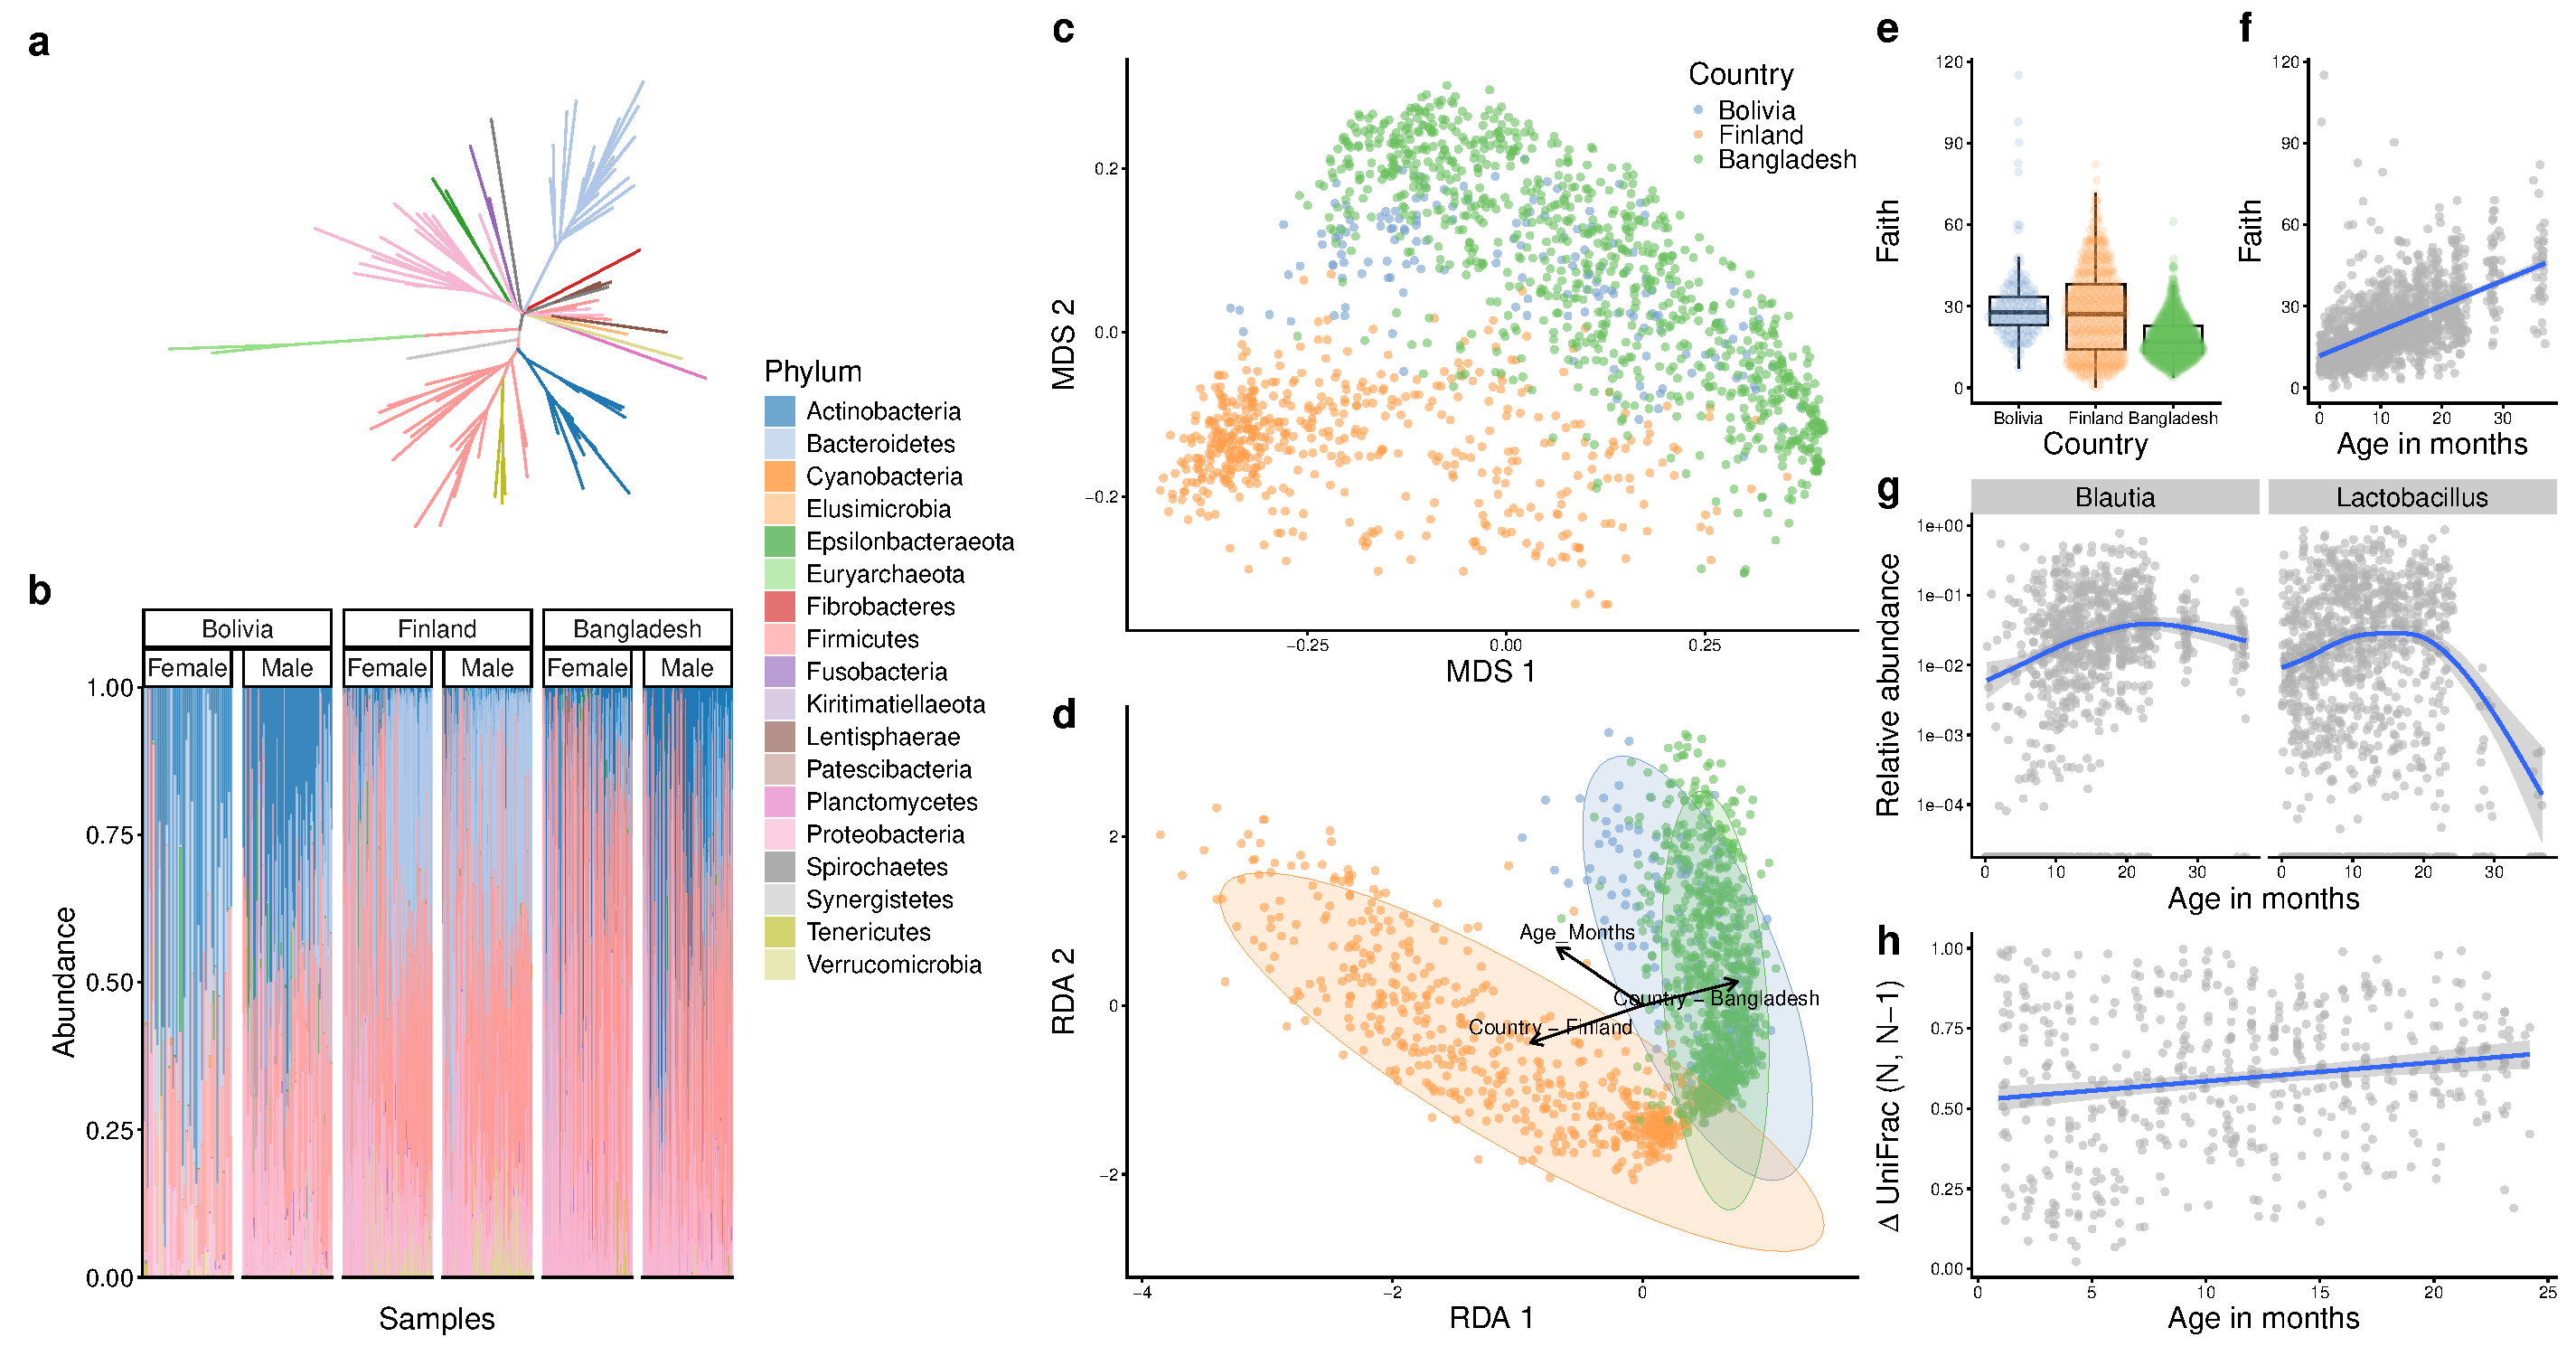
\includegraphics[keepaspectratio]{manuscript_files/figure-pdf/fig-downstream_analyses-1.pdf}}

}

\caption{\label{fig-downstream_analyses}\textbf{Common visualization
methods.} This set of visualizations present time series data on infants
from three different countries. \textbf{Figure A} illustrates the
phylogenetic relationships, while \textbf{Figure B} summarizes phyla
abundances in the samples ordered based on age. Actinobacteria is more
present in Bolivia and Bangladesh compared to Finland. \textbf{Figures C
and D} display the results of Multidimensional Scaling (MDS) using
Unifrac distances and Distance-based Redundancy Analysis (dbRDA) based
on Aitchison distance, respectively. Both ordination methods shows clear
pattern separating microbial profiles in different countries. dbRDA
shows additionally association between microbial profile and age.
\textbf{Figures E and F} depict Faith's phylogenetic diversity
visualized in respect to country and age. \textbf{Figure G} visualizes
Differential Abundance Analysis (DAA) results with scatter plot. Two
genera exhibit association with age. \textbf{Figure H} illustrates
Unifrac divergence for consecutive time points. Results indicate slow
stabilization of microbial communities.}

\end{figure}%

\section{Accessible analysis and community}\label{sec-community}

Modern science is embodied by a critical community capable of assessing
discoveries and replicating results \citep{Wootton2016}. Open software
and the social structures around it present a timely manifestation of
this principle, with technical, legal, sociological and epistemic
consequences \citep{Hocquet2024}. FAIR principles for software support
access to well-documented and user-friendly methods \citep{Barker2022},
and these are facilitated by the extensive quality control and
documentation standards enforced by Bioconductor \citep{huber2015}. In
addition to these technical demands, the development and quality control
of academic software critically relies on active critical source
communities that can provide continuous benchmarking and support the
identification and dissemination of evidence-based best practices
\citep{berg2020, Barker2022, Hocquet2024}. We actively support community
formation by online training resources and communication channels.
These, together with the interactive applications, provide accessible
entry points for prospective developers and users.

\textbf{The OMA book.} \emph{Orchestrating Microbiome Analysis with
Bioconductor (OMA)} (https://microbiome.github.io/OMA/docs/devel/) is an
online book that provides a comprehensive introduction to the microbiome
data science framework in Bioconductor. It offers practical guidance,
reproducible workflows, and training material for integrative microbiome
analyses. The book is versioned to match Bioconductor's biannual
software release cycles. The work incorporates rich feedback from the
user community and microbiome training courses. It complements the
broader trend, where specific Bioconductor data structures
\citep{huber2015, ramos2017, huang2021} have been adopted as a solution
for multi-table data integration tasks in various domains such as
single-cell sequencing (OSCA book) \citep{amezquita2020} and
transciptomics \href{https://lmweber.org/OSTA/}{OSTA book}. These
resources demonstrate how state-of-the-art data containers can support
statistical programming on interlinked multi-table data sets in a highly
optimized way.

\textbf{Interactive applications.} Graphical user interfaces provide
accessible entry points to the framework. The iSEEtree and miaDash
packages provide interactive analysis and visualization tools for
microbiome data \citep{benedetti2025}
(Figure~\ref{fig-downstream_analyses}). Their interface supports
automatic generation of source code and replicable workflows as well as
analysis templates for users without a strong programming expertise.
Moreover, the tidy R paradigm, available through tidyomics, simplifies
the syntax and can streamline the workflows \citep{hutchison2024}. These
tools allow users to perform basic analyses and visualize data with
ease.

\textbf{Community.} Its widespread adoption has made R one of the most
cited software resources of our time \citep{Pearson2025} and the
introduction of the shared data structures facilitates the broad
interoperability of the methods ecosystem. Bioconductor has a strong
tradition in fostering the R user community through shared data
structures and training activities \citep{drnevich2025}. An active
community of developers and users thrives online, supporting the
software sustainability and promoting good practices in scientific
computing \citep{Wilson2017}. The community interacts via several online
communication channels, including Bioconductor Zulip, Github forum, and
an email list. The development of the framework is influenced by
feedback from the user community through these channels, regular
meetings and training workshops.

\section{Outlook}\label{sec-discussion}

\textbf{The Bioconductor community} has a well-established reputation in
developing open, peer-reviewed software for life sciences. Its strengths
include the enforcement of minimal documentation standards, semantic
versioning, portability across operating platforms, quality control
(e.g.~unit testing, continuous integration), usability (APIs), and
robustness (deprecation mechanisms), and a biannual release cycle.
During the past two decades Bioconductor has grown into a repository of
2,300 actively maintained software packages, of which 58 are classified
under the Microbiome Bioc task view. In order to enjoy the benefits of
automation while maintaining flexibility, data scientists routinely
remix open-source software into custom workflows. However, the lack of
commonly adopted data representation standards often hinders the
development, sharing, and application of statistical workflows. At the
core of the Bioconductor's data science strategy is the idea of shared
data representation. The enhanced interoperability can help to minimize
redundant efforts and facilitate the translation of methods between
different research areas \citep{DElia2023, Barker2022} and, importantly,
facilitates the formation of broad developer and user communities.

\textbf{Microbiome research} has shifted towards integrative analyses
aiming at mechanistic and causal inference
\citep{joos2024, bastiaanssen_bugs1_2023}. Technological advances in
long-read sequencing, functional assays, spatial profiling, and
single-cell have created an increasing demand for integrative data
analysis techniques. Thus, microbiome data is increasingly linked with
other omics along varying spatial and temporal dimensions. Our framework
addresses this need, together with parallel developments in other areas
of omics.

Recent developments in microbiome and multi-omics workflows increasingly
rely on Bayesian modeling and Gaussian processes to accommodate
uncertainty and temporal or spatial structures \citep{cheng2019}. Our
framework is compatible with these approaches, providing the structured
input necessary for probabilistic inference and scalable computation.
Building on these statistical foundations, the rapid emergence of
foundation models and deep learning approaches in biomedicine calls for
robust, scalable data representations \citep{awais2025}. Our framework,
through its use of standardized containers and modular workflows, is
well-positioned to support such advances. Applications include transfer
learning across studies, interpretable embeddings of microbiome
multi-omic profiles, computational prediction of microbial function and
metabolites \citep{mallick2019, weiss2016}, and integration with AI
agents for hypothesis generation and automated analysis, among others
\citep{zou2025, gao2024}.

\textbf{Open data science infrastructures} have become critical
components of reproducible research and a vast body of applications
critically rely on open-source methods and workflows
\citep{berg2020, Barker2022, Hocquet2024}. Standardized data structures
can enhance the transparency, reliability, and explainability of
analysis workflows. We have documented the interoperable framework built
on widely adopted data containers, open data resources, analysis methods
and reproducible workflows for multi-modal microbiome research. Further
developments could include extended methodology for temporal, spatial,
and multi-omic analyses. Supporting interoperability between R and other
programming languages can facilitate the application of other ML
frameworks. As the field evolves, Bioconductor will continue to
integrate new tools and approaches to improve integrative analyses of
microbiome data.

\section{References}\label{references}

\renewcommand{\bibsection}{}
\bibliography{bibliography.bib}

\subsection{Consortia}\label{sec-consortium}

Mia Contributors: \textbf{we will list here main and consortium authors
who approved their inclusion} on
\href{https://docs.google.com/spreadsheets/d/1r6eiWS1yT2kDHvnez5uklcI5kDXrPGm-v252-eC1C_Y/edit?gid=1938866487\#gid=1938866487}{this
sheet}. Sorted in alphabetical order by last name.

\subsection{Contributions}\label{sec-contributions}

LL and TB initiated and coordinated the work. All authors contributed
material, participated the manuscript preparation, and approved the
final version.

\subsection{Acknowledgments}\label{sec-acknowledgments}

This project received funding from the European Union's Horizon 2020
research and innovation programme under grant agreement No 952914. TB
was additionally supported by the University of Turku Graduate School.

We would like to thank the following individuals for their support for
the project: Richa Ashma, Nitin Bayal, Chouaib Benchraka, Axel Dagnaud,
Teo Dallier, Noah de Gunst, Karoline Faust, Samuel Hillman, Hervé Pagés,
Mahkameh Salehi, Daniel Rios Garza, Matti Ruuskanen. We also extend our
thanks to all contributors of the open-source resources used in this
work.





\end{document}
